
% [[file:e:/projects/software/reproducible_research/slides/p_repro_research.org::*What%20a%20Sweave%20file%20looks%20like][What-a-Sweave-file-looks-like:1]]

%% filename: src/tex/examp_sweave-01.Rnw
\documentclass[noae]{article}

\usepackage[utf8x]{inputenc}
\usepackage[T1]{fontenc}
\usepackage[english]{babel}
\usepackage[margin = 1in]{geometry}

\title{This is a tiny Sweave example}
\author{Bernd Weiss}

\usepackage{Sweave}
\begin{document}
\maketitle

I am using a built-in dataset which is called \texttt{USArrests} 
(Violent Crime Rates by US State).

\begin{Schunk}
\begin{Sinput}
> summary(USArrests)
\end{Sinput}
\begin{Soutput}
     Murder          Assault         UrbanPop          Rape      
 Min.   : 0.800   Min.   : 45.0   Min.   :32.00   Min.   : 7.30  
 1st Qu.: 4.075   1st Qu.:109.0   1st Qu.:54.50   1st Qu.:15.07  
 Median : 7.250   Median :159.0   Median :66.00   Median :20.10  
 Mean   : 7.788   Mean   :170.8   Mean   :65.54   Mean   :21.23  
 3rd Qu.:11.250   3rd Qu.:249.0   3rd Qu.:77.75   3rd Qu.:26.18  
 Max.   :17.400   Max.   :337.0   Max.   :91.00   Max.   :46.00  
        Murder_d    UrbanPop_d
 (0.8,7.25] :24   (32,66]:25  
 (7.25,17.4]:25   (66,91]:24  
 NA's       : 1   NA's   : 1  
\end{Soutput}
\end{Schunk}

The mean for "Murder arrests (per 100,000)" is 7.788.

\setkeys{Gin}{width=0.4\textwidth}

\begin{figure}[h!]
\begin{center}
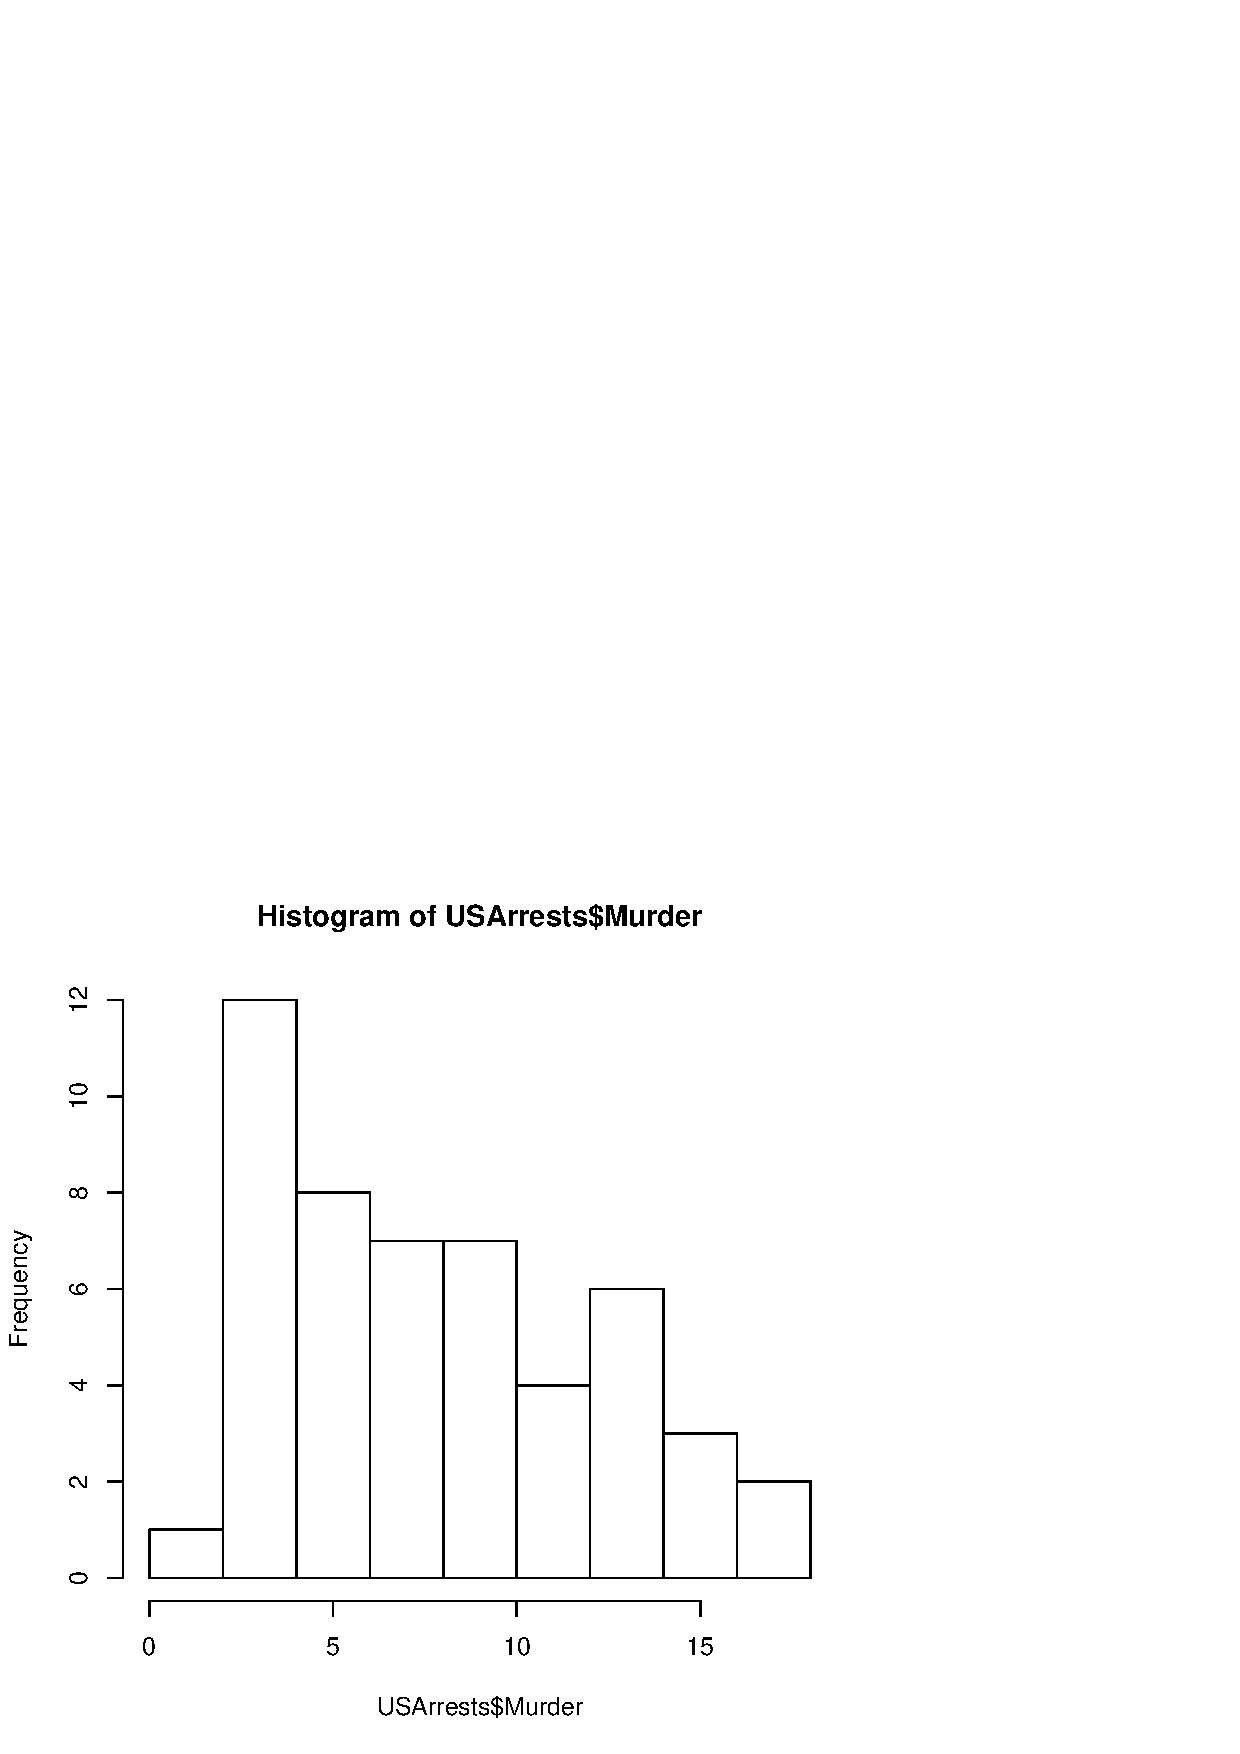
\includegraphics{examp_sweave-01-002}
\end{center}
\caption{Murder arrests (per 100,000)}
\end{figure}

\end{document}

% What-a-Sweave-file-looks-like:1 ends here
